\documentclass[11pt]{article}
\setlength{\topmargin}{-0.8in} % usually -0.25in
\addtolength{\textheight}{1.4in} % usually 1.25in
\addtolength{\oddsidemargin}{-0.8in}
\addtolength{\evensidemargin}{-0.8in}
\addtolength{\textwidth}{1.6in} %\setlength{\parindent}{0pt}

\usepackage[T1]{fontenc} % Recommended for better encoding
\renewcommand{\familydefault}{\sfdefault}
\usepackage{helvet}

% macros
\usepackage{amsmath,
amssymb,
mathrsfs,
amsthm,
fancyhdr,
tikz,
multicol,
enumitem
}

\newcommand{\be}{\begin{enumerate}}
 \newcommand{\ee}{\end{enumerate}}


\newcommand{\C}{{\mathbb{C}}}
\newcommand{\R}{{\mathbb{R}}}
\newcommand{\eps}{\epsilon}
\newcommand{\Z}{{\mathbb{Z}}}
\newcommand{\Q}{{\mathbb{Q}}}
\newcommand{\N}{{\mathbb{N}}}



\lhead{{Math 265 Proofs}}
\chead{\large \ Midterm I (Solutions)} 
\rhead{Spring 2026}
\cfoot{}
\pagestyle{fancy}
\begin{document}
\thispagestyle{fancy}
\begin{enumerate}
%Set builder notation
\item (8 pts) Write the set using \textbf{set builder} notation.
		\be
		\item $\{ \dots, -10, -6, -2, 2,6,10, 14, 18, \dots \}$ (Assume the pattern continues.)\\
		$\{ 4n+2 : n \in \Z\}$
		\vfill
		\item The set of real numbers whose squares are integers.\\
		$\{ x \in \R : x^2 \in \Z\}$
		\vfill
		\ee
% element subset distinction
\item (10 pts) Consider the set $A=\big\{ 1, \, 2, \, 3, \, \{2\}, \, \{2,3\},\,  \{ 1, \{1\}\}\,  \big\}$
	\be
	\item The cardinality of $A$ is 6.\\
	
	
	\item Determine if the statements below are true or false.
		
		\begin{multicols}{2}
		\be[leftmargin=0cm]
		\item $\emptyset \in A$ \quad False\\		
		\item $\emptyset \subseteq A$ \quad True \\
		\item $1 \in A$ \quad True\\
		\item $1 \subseteq A$ \quad False\\
		\item $\{1\} \in A$ \quad False\\
		\item $\{1\} \subseteq A$ \quad True\\
		\item $\{1,\{1\}\} \subseteq A$ \quad False\\
		\item $\{2,\{2\}\} \subseteq A$ \quad True\\
		\ee
		\end{multicols}
	\ee

%power set and cartesian product
\item (10 pts) Consider the set $B=\{ n^2 \, : \,  n \in \Z \text{ and } |n| \leq 3 \}$
	\begin{enumerate}
	\item Rewrite the set $B$ by listing its elements between braces.\\ 
	$\{0,1,4,9\}$
	\item  $\big\vert\mathcal{P}(B)\big\vert = $ \underline{$2^4=16$} (where $\mathcal{P}(B)$ is the power set of $B.$)
	\item Show that the following statement is true: $$\exists X_1\in \mathcal{P}(B), \exists X_2 \in \mathcal{P}(B), \,0 < |X_1| < |X_2| \text{ and } X_1 \cap X_2 = \emptyset.$$
	Choose $X_1=\{0\}$ and $X_2 = \{1,4\}$.
	\item $\big\vert B \times B \big\vert=$ \underline{$4 \cdot 4=16$}	
	\item Let $D=\{ (a,b) \in B \times B \, : \, a+b=1\}.$ Rewrite the set $D$ by listing its elements between braces.\\
	$\{ (1,0), (0,1)\}$
	\vfill
	\ee
%union and complement
\item (10 pts) Let $A=\{ (x,y) \in \R \times \R \, : \, y \leq 1\}$, $B =\{ (x,y) \in \R \times \R \, : \, y \geq x^2\}$, and the universal set, $U=\R \times \R,$ the entire $xy$-plane. Sketch each set below. Clearly label your pictures.
	\begin{multicols}{2}
	\be
	\item $A \cap B$\\
	
	\begin{tikzpicture}[scale=1.2]
    % Draw axes
    \draw[->] (-1.8,0) -- (1.8,0) node[right] {$x$};
    \draw[->] (0,-0.5) -- (0,2) node[above] {$y$};
    
    % Fill the intersection region (below y=1 AND above y=x²)
    \fill[blue!30, domain=-1:1, samples=100] 
        plot (\x, {\x*\x}) -- (1,1) -- (-1,1) -- cycle;
    
    % Draw the parabola y = x²
    \draw[thick, dashed, domain=-1.25:1.25, samples=100] 
        plot (\x, {\x*\x}) node[right] {$y = x^2$};
    \draw[thick, domain=-1:1, samples=100] 
        plot (\x, {\x*\x});
  
    % Draw the line y = 1
    \draw[thick, dashed, domain=-1.5:1.5] 
        plot (\x, 1) node[right] {$y = 1$};
     \draw[thick,  domain=-1:1] 
        plot (\x, 1);
   % Add labels
    \node at (0, 0.5) {$A \cap B$};
\end{tikzpicture}

	\item $ \overline{A} \cup B$
	
\begin{tikzpicture}[scale=1]
    % Draw axes
    \draw[->] (-1.8,0) -- (1.8,0) node[right] {$x$};
    \draw[->] (0,-0.5) -- (0,2.5) node[above] {$y$};
    
    % Fill A̅ (complement of A, which is y > 1)
    \fill[gray!20] (-1.8,1) rectangle (1.8,3);
    
    % Fill B (y ≥ x²) - the region above the parabola
    \fill[gray!20, domain=-1:1, samples=100] 
        plot (\x, {\x*\x}) -- (-1,1) -- (1,1) -- cycle;
    
    % Draw the parabola y = x²
    \draw[ultra thick, domain=-1.5:1.5, samples=100] 
        plot (\x, {\x*\x}) node[right] {$y = x^2$};
    
    % Draw the line y = 1
    \draw[ultra thick, dashed, domain= -1.8:-1] 
        plot (\x, 1) {};
    \draw[ultra thick,dashed, domain=1:1.8] 
        plot (\x, 1) node[right] {$y = 1$};
    
    % Add title
    \node at (0, -1) {(b) $\overline{A} \cup B$};
    
    % Add labels
    \node at (0, 2) {$\overline{A} \cup B$};
\end{tikzpicture}
	
	\ee
	\end{multicols}
	\vfill
	\vfill
\item (12 pts) For any number $n,$ let $A_n = [0,\frac{n}{n+1}].$ Determine the following subsets of the real line.
	\begin{multicols}{2}
	\be
	\item $A_1=$ \underline{$[0,\frac{1}{2}]$}\\
	
	\item $A_2=$ \underline{$[0,\frac{2}{3}]$}\\
	
	\item $A_3=$ \underline{$[0,\frac{3}{4}]$}\\
	
	\item $\displaystyle\bigcap_{n \in \N} A_n=$ \underline{$[0,\frac{1}{2}]$}\\
	
	\item $\displaystyle\bigcup_{n \in \N}  A_n=$ \underline{$[0,1)$}\\

	\ee
	\end{multicols}

%% Write If-Thens
\item (12 pts) Rewrite each sentence below in the form ``If $P$, then $Q.$"
	\be
	\item In order for Rachel to wear black, it is necessary that it is a Tuesday.\\
	
	If Rachel wears black, then it is Tuesday.\\
	
	\item The presence of a full moon is sufficient for the flower to bloom.\\
	
	If there is a full moon, then the flower will bloom.
	
	\item The card is an ace only if the table is flat.\\
	
	If the card is an ace, then the table is flat.
	
	\item The blueberries are ripe or the cranberries are ripe.\\
	
	If the blueberries are not ripe, then the cranberries are ripe.
	\ee
%% english to logic, negations, back to english
\item (15 pts)  For parts (a) and (b): (i) rewrite the given statement symbolically and, then,  (ii) negate it.  
	\be
	\item For every subset $X$ of $\N$ there is always another subset $Y$ of $\N$ such that $X\not = Y$ and $ X \subseteq Y.$\\
		\be[leftmargin=0cm]
		\item symbolic form: $\forall X \subseteq \N, \exists Y \subseteq \N, (X\not = Y) \land (X \subseteq Y)$\\
		
		\item negation: $\exists X \subseteq \N, \forall Y \subseteq \N, (X= Y) \lor (X \not \subseteq Y)$\\
		
		\ee
	
	\item For every $\epsilon > 0$, there is a $\delta >0$ such that if $|x-a| < \delta$ and $x \not = a,$ then $|f(x)-L| < \epsilon.$ (Note: The function $f(x)$ is fixed and $a$ and $L$ represent fixed constants.)
		\be[leftmargin=0cm]
		\item symbolic form: $\forall \epsilon > 0, \exists \delta > 0, \forall x \in \R, \big( (|x-a| < \delta) \land (x \not = a)\big) \Rightarrow (|f(x)-L| < \epsilon)$ \\
		\vspace{.5in}
		
		\item negation: $\exists \epsilon > 0, \forall \delta > 0, \exists x \in \R, \big( (|x-a| < \delta) \land (x \not = a) \land (|f(x)-L| < \epsilon)\big)$\\
		\vspace{.5in}
		\ee

	\item Determine if the statement in part (a) is true or false. Justify your answer.\\
	
	It is false. Or, equivalently, its negation is true. Specifically, if we select $X=\N$, then for every subset $Y$ of $\N,$ $Y = X$ or not. If $Y=X,$ then the negation is true. If $Y \not = X,$ then $X$ necessarily contains an element that $Y$ does not. Thus, $X \not\subseteq Y.$
		\vfill
	\ee
\item(8 pts) Show that the statements \fbox{$(P \Rightarrow Q) \Rightarrow R$} and \fbox{$(P \land Q) \lor R$} are \textbf{not} logically equivalent.\\

It is sufficient to find truth values for $P, Q,$ and $R$ such that the statements have different values. \\

Choose $P=\text{true}, Q=R\text{false}.$ \\

Then the second one,  \fbox{$(P \land Q) \lor R$}, is false since $R$ is false by choice and $P \land Q$ is false since $T \land F =F.$\\

On the other hand, $(P \Rightarrow Q) =F$ since the hypothesis is true and the conclusion is false. Thus, the first statement now has the form $F \Rightarrow T=T.$
\vfill

%% Truth table + valid argument
\item (15 pts) \textbf{Use a truth table} to determine whether the argument below is valid or invalid. \textbf{Your answer must include:}
\be
\item[(a)] A complete truth table with clearly labeled columns.
\item[(b)] An explanation of how the truth table demonstrates whether the argument is valid or invalid
\ee

\textbf{Note:} Organize your work clearly. Points will be deducted for poor organization.\\

\begin{tabular}{c}
$P \: \Rightarrow \: R$ \\
$Q \: \Rightarrow \: R $ \\
\hline
$\therefore \: P \lor Q \Rightarrow \: R$ \\
\end{tabular}
%\begin{center}
\begin{tabular}{|c|||c|c|c|c|c|c|c|}
\hline
&1&2&3&4&5&6&7\\
row&$P$ & $Q$ & $R$ & $P \Rightarrow R$ & $Q \Rightarrow R$ & $(P \lor Q)$ & $(P \lor Q) \Rightarrow R$ \\
\hline
a&T & T & T & T  & T & T & T \\
b&T & T & F & F & F & T  & F\\
c&T & F & T & T & T & T &  T\\
d&T & F & F & F & T & T &  F\\
e&F & T & T & T & T & T &  T\\
f&F & T & F & T & F & T &  F\\
g&F & F & T & T & T & F &  T\\
h&F & F & F & T & T & F & T \\
\hline
\end{tabular}
%\end{center}

There are five rows (a,c,e,g,h) where both hypotheses (columns 4 and 5) are true. For each of these five rows, column 7 is also true. This demonstrates that the argument is valid.


\end{enumerate}
\end{document}